% !TeX spellcheck = en_US
% This template is a derived work from "LaTeX Example: Project Report: http://www.howtotex.com"

\documentclass[paper=a4, fontsize=11pt, titlepage]{scrartcl}
\usepackage[T1]{fontenc}
\usepackage{fourier}
\usepackage[english]{babel}	
\usepackage[protrusion=true,expansion=true]{microtype}	
\usepackage[latin1]{inputenc}
\usepackage{amsmath}
\usepackage{amsfonts}
\usepackage{amssymb}
\usepackage{listings}
\usepackage[pdftex]{graphicx}
\usepackage{glossary}
\usepackage[hyphens]{url}
\bibliographystyle{alpha}

%%% Custom sectioning
\usepackage{sectsty}
\allsectionsfont{\centering \normalfont\scshape}

\setlength{\headheight}{13.6pt}

%%% Equation and float numbering
\numberwithin{equation}{section}		% Equationnumbering: section.eq#
\numberwithin{figure}{section}			% Figurenumbering: section.fig#
\numberwithin{table}{section}			% Tablenumbering: section.tab#

% Horizontal rule
\newcommand{\HRule}[1]{\rule{\linewidth}{#1}}

% New command: footnote reference, to point to an existing footnote
\makeatletter
\newcommand\footnoteref[1]{\protected@xdef\@thefnmark{\ref{#1}}\@footnotemark}
\makeatother

\begin{document}

	% This is a derived work from 
% http://en.wikibooks.org/wiki/LaTeX/Title_Creation#A_practical_example

\begin{titlepage}
\begin{center}


\includegraphics[width=0.15\textwidth]{img/logo.pdf}
~\\[1cm]
\textsc{\LARGE Free University of Bolzano/Bozen}
\\[1.5cm]
\textsc{\Large CASE Report}
\\[0.5cm]

% Title
\HRule{0.5pt} 
\\[0.4cm]
{ 
	\huge 
	\bfseries 
	Integration of PROM framework with SonarQube and Atlassian Jira Agile \\[0.4cm] 
}
\HRule{2pt} 
\\[1.5cm]

% Author and supervisor
\noindent
\begin{minipage}{0.4\textwidth}
	\begin{flushleft} \large
		\emph{Author:}\\
		Peter \textsc{Moser}
	\end{flushleft}
\end{minipage}%
\begin{minipage}{0.4\textwidth}
	\begin{flushright} \large
		\emph{Submitted to:} \\
		Prof.~Alberto \textsc{Sillitti}
	\end{flushright}
\end{minipage}


\vspace{2cm}

{\large \today}

% Bottom of the page
\vfill

\HRule{0.1pt} 
\\[0.2cm]
\begin{flushleft}
This document investigates on what PROM could add to SonarQube and Atlassian
Jira. First, I start from what SonarQube already supports. Second, I describe
what PROM can add to their functionalities, that is, what are possible features
of PROM that could improve their economic value. Afterward, I repeat both steps
for Atlassian Jira, especially for Jira Agile. Please notice, that I write this
report in a non-official manner, such that I can seed random thoughts on how we
could integrate PROM in both third-party tools.
\end{flushleft}
\HRule{0.1pt}
\end{center}
\end{titlepage}
	
	\tableofcontents
	
	\section{SonarQube}
\subsection{What does SonarQube provide?}
SonarQube offers product metrics for various languages: ABAP, Android, C/C++,
C-Sharp (C\#), COBOL, Flex, Groovy, Java, JavaScript, Objective-C, PHP, PL/I,
PL/SQL, Python, RPG, VB.NET, Visual Basic 6, Web (HTML, JSP/JSF), and XML. In
addition to build-in functionalities, plugins allow for multi-language analysis
of code
quality\footnote{\url{http://www.sonarqube.org/at-long-last-sonarqube-is-a-true-polyglot/}}.
It is even possible to compare metrics between different languages and projects,
i.e. side by side comparison between Java and C++.

These are the product metrics currently supported by SonarQube (formerly known
as Sonar)\footnote{\url{http://docs.codehaus.org/display/SONAR/Metric+definitions}}:
\begin{itemize}
	\item \textbf{Cyclomatic Complexity}: overall, and average by class, file and function.
	\item \textbf{Design issues}: 
	\begin{itemize}
		\item cycles, file cycles, file dependencies, and package edge weight, 
		that is, number of dependencies between packages
		\item Depth of inheritance tree (tic)
		\item Number of children (noc) of a class
		\item Response for class (rfc) 
		\item Afferent and efferent couplings (ca, ce): how many classes use 
		this class, or how many classes are used by this class
		\item Lack of cohesion of methods (lcom4), i.e. set of related 
		components of a class. There should be only one, otherwise the class should be divided into smaller classes.
	\end{itemize}
	\item Duplications of source code blocks and lines.
	\item Metrics about issues: open, confirmed, closed, false positive.
	\item Metrics about defined rule compliance, i.e. violation density. \\
	Violations is the number of rule breaches automatically calculated by
	analyzing the source code of a project. Different projects can be compared to each other. In addition, developers can weight violations to find out where they must start fixing problems first.
	\item Technical debt is the effort to fix all issues in minutes.
	\item Severity of issues is calculated automatically through defined rules,
	several rule packages already exist for different languages, and are bundled
	together with the default installation.
	\item Size metrics: LLOC, LOC, generated LOC, method counts, class counts, 
	file counts, public API, and statements.
	\item Test metrics: condition coverage for branching code, and separately 
	for new code, and line coverage. Further more it exists a unit test 
	integration with duration, errors, failures, and success density.
	\item Documentation metrics: lines of comments, significant lines of comments, commented out production code, and Javadoc support.
	\item Source code repository metrics about commits, revisions, and authors'
	performance.
\end{itemize}

According to~\cite{Gallaba} the most important metrics are: duplicated blocks, violations,
public undocumented APIs, uncovered complexity by tests, function and class
complexity distribution, and package edge weights.
The overall measures of these metrics are used to calculate the technical debt
in man days:

\begin{align}
\begin{split}
\label{Technical debt in man days}
technical\_debt = & cost\_to\_fix\_duplications + \\
  	& cost\_to\_fix\_violations + \\
  	& cost\_to\_comment\_public\_API + \\
  	& cost\_to\_fix\_uncovered\_complexity + 	\\
  	& cost\_to\_bring\_complexity\_below\_threshold +\\
  	& cost\_to\_cut\_cycles\_at\_package\_level
\end{split}
\end{align}

This technique is known as SQALE Rating\footnote{\url{http://docs.codehaus.org/display/SONAR/Technical+Debt#TechnicalDebt-ComparingprojectswiththeTechnicalDebtRatioandtheSQALERating}}. Technical debt ratio, that is shown in
figure 2 and figure 5, is calculated with the following formula:

\begin{equation}
\label{Technical Debt Ratio}
technical\_debt\_ratio = technical\_debt / estimated\_development\_cost
\end{equation}


In addition to these metrics, SonarQube provides Eclipse and IntelliJ plug-ins to
handle issues directly from within the IDEs. It also harvests some state of the
art issue tracker currently available on the market, i.e. JIRA issues, Trac,
Mantis Bug Tracker\footnote{MantisBT is an open source issue tracker:
http://www.mantisbt.org/}. There exist also plugins to seamlessly include other
test and metric environments, like the Apache JMeter
plugin\cite{http://docs.codehaus.org/display/SONAR/JMeter+Plugin} to test
performance of
static and dynamic resources, or Pitest\footnote{PIT is a mutation testing tool for
java: http://pitest.org/} to handle mutation testing.

\subsection{What can PROM get from SonarQube or add to it?}

As what I have seen so far, SonarQube is mainly focused on product metrics and
issue tracking environments, i.e. bug reports and task lists. However, I think
it has no effort collection system, since these information is always given
manually by developers. They insert estimates and progressions by hand into
software development management tools, that are harvested later by the SonarQube
analyzing tools, like SonarQube Runner, SonarQube Ant Task, Maven or Gradle
Engines\footnote{How Sonar analyzes source code: http://docs.codehaus.org/display/SONAR/Analyzing+Source+Code}.

I put the focus to the SonarQube Runner tool for the moment, since it is the
recommended analyzer.  This tool analyzes a project and puts all calculated
metrics into a specified database. 

First, we could use this data to enhance PROM's feature list, with the metrics
mentioned earlier in this document.
Second, PROM could add real-time effort data to imported task structures and
issues. That is, combine effort accumulated by a developer per task. These tasks
could then, also with PROM, be combined with source code fragments, i.e.
classes, methods, name spaces, and projects. The capability of SonarQube to
provide a list with the most critical project components, that is components
that have a high probability to fail, combined with real effort data connected
to them, could provide powerful statistics. For example, if a developer
estimated a task with X man days and worked on it for a certain time Y, an
effort analysis plug-in that accesses PROM data, could provide real-time
''technical debt'' or ''print completion'' (i.e., for SCRUM methodology)
statistics. On one hand, we could provide such statistics for tasks and issues.
On the other hand, we could provide them for source code fragments.

Another feature, that we could use to extend PROM, are source code complexity
metrics. The PROM team implemented some metrics for source code analysis. These
are, CBO (coupling between objects),  CC (cyclomatic complexity), DIT (Depth of
Inheritance Tree), LCOM (lack of cohesion of methods), NOC (number of children),
RFC (response set of a class), and WMC (weighted methods for class), and more
direct metrics like LOC, and LLOC. However, these metrics work only (as I know)
for Java and C++. SonarQube provides most of these metrics for a broad variety
of languages, as you can see in figure 6.

\subsection{Suggestions for plug-ins}

\subsubsection{First plug-in: Combine effort data with source code}

First, I would suggest to integrate non-invasive effort metrics to projects that
SonarQube manages. That is, map effort to source code fragments. 

A possible outcome could be a table that shows the overall effort of a project,
and on higher granularity it provides effort subdivided into name spaces,
classes, and methods. Since SonarQube allows to import source code from revision
control systems, like GIT or SVN, it would be important to add revisions to such
metrics as well. This is, as I know, not implemented yet for PROM.

\subsubsection{Second plug-in: Combine effort data with tasks and issues}

Second, I would suggest to create a visualization plug-in that shows non-invasive
effort metrics per task and issue. We could also add PERT or GANTT to gain
additional value. To provide a professional state-of-the-art tool, that supports
third-party products we could also create an export function, i.e. for Microsoft
Project. However, SonarQube is an open-source tool, I think it would be better
to export data to other open-source management tools, like GanttProject. I have
done such a project for my Bachelor thesis. It is possible to reuse this as a
SonarQube plugin.

\subsubsection{Third plug-in: Integrate PROM's GQ(I)M dashboard}

Third, SonarQube has no support for a GQM dashboard. I think, developers will
appreciate if we create a SonarQube GQ(I)M dashboard to visualize their
statistics enriched with our effort metrics. 

All three plugins could be combined to a PROM suite for SonarQube. In general,
we should provide some REST interface, to simply query PROM's effort collections
according to certain filters and constraints. However, this would involve some
major project changes and improvements.

	% !TeX spellcheck = en_US
\section{Atlassian Jira Agile}
\subsection{What does Jira Agile provide?}

Jira Agile provides task management support for the two main agile methodologies
SCRUM and Kanban. It focuses on creating and managing tasks, issues, stories,
epics and bug reports. Developers can estimate and prioritize these planning
cards. Administrators define task flow processes according to certain filters
and constraints. All developers must follow these rules afterward. The whole
Jira framework is highly adaptable and configurable to future needs, i.e. new
Kanban board columns and statuses can be defined and multiple projects can be
visualized all at once on a configurable dashboard. It also integrates with
Jira, Confluence and other development tools. 

Another feature is the integration with source code revision tools, like Git,
SVN and Bitbucket. It bridges the gap between user stories and source code
commits.

On the side of analysis, Jira Agile does not offer a lot. At least build-in features are scarce. If developers use Kanban, they can monitor current trends and analyze past progresses. The tool that visualizes this metrics is called cumulative flow diagram, please refer to figure~\ref{fig:cumulative_flow_diagram}. I think, this could be a good point where PROM comes in with analysis tools. Maybe we could add effort metrics and product metrics here. For instance, CC, LLOC, and LCOM4. It could be even feasible to integrate SonarQube features here, maybe we could add them first to PROM services, or provide an unified interface to PROM and SonarQube metrics and statistics through a REST service or something similar.

\begin{figure}[h]
	\centering
	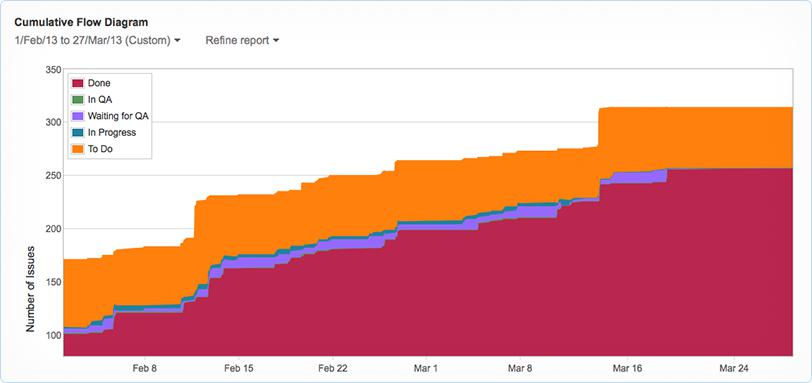
\includegraphics[scale=0.5]{img/cumulative_flow_diagram.jpg}
	\caption{Cumulative flow diagram with number of issues over time.} 
	\label{fig:cumulative_flow_diagram}
\end{figure}

Although, Atlassian Jira comes with some experimental advanced report features, that a developer can enable through a simple click. In general, users can define filters to refine charts and reports. It is possible to zoom in and out charts and move along the axis with the mouse pointer to get additional information about a certain point in time.

From our perspective, in order to add some value to these reports and charts, PROM could provide real-time effort statistics. However, I do not know now if it is possible to add functionality to these charts directly, or if it would be necessary to write a plug-in from scratch that visualizes such data enriched with our effort collections.

The following list shows the most important report types, gives a fast insight to their functionality, and screenshots. I will not provide full description to these, due to a more complete manual available online\footnote{\label{fn:report_modes}\url{https://confluence.atlassian.com/display/AGILE063/Using+Report+Mode}}. Since I am concerned about Jira Agile, I will describe only report types that match the criteria of agile methodologies. Also Jira does the same, since it excludes automatically all issues and data fields, that do not belong to a certain board type, i.e. Kanban board, and Scrum board.

The following reports and charts are available\footnoteref{fn:report_modes}:

\begin{itemize}
	\item Control Chart
	\item Burndown Chart (for Scrum boards only)
	\item Cumulative Flow Diagram
	\item Epic Report (for Scrum boards only)
	\item Sprint Report (for Scrum boards only)
	\item Velocity Chart (for Scrum boards only)
	\item Version Report (for Scrum boards only)
\end{itemize}

\textbf{Control chart}: A control chart can show the cycle time or lead time for your product, version or sprint. The horizontal x-axis in a Control Chart indicates time, and the vertical y-axis indicates the number of days issues have spent in those statuses.

\begin{figure}[h]
	\centering
	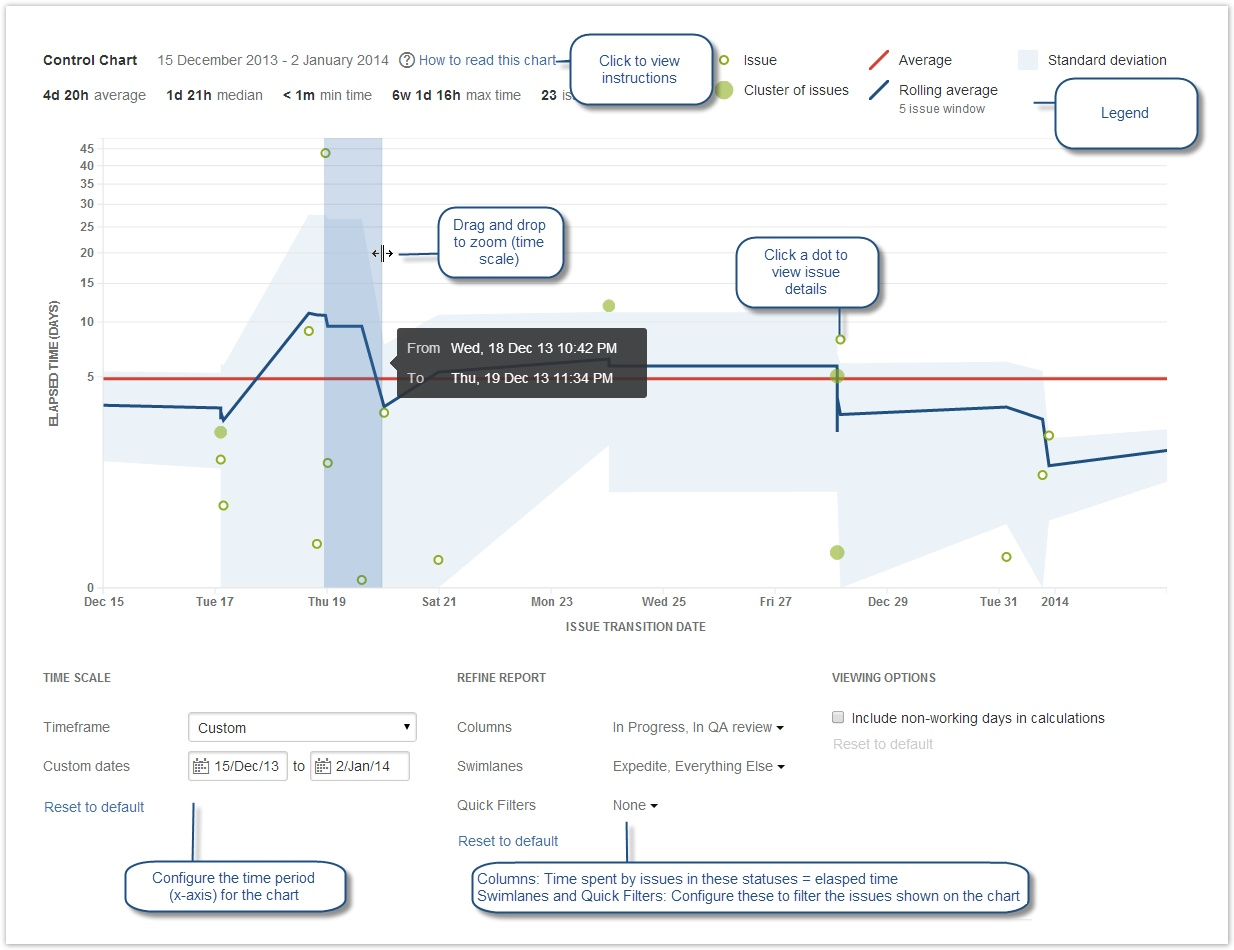
\includegraphics[scale=0.4]{img/agile-controlchart-annotated.jpg}
	\caption{Screenshot: Control Chart with annotations.} 
	\label{fig:agile-controlchart-annotated}
\end{figure}

\textbf{Burndown chart}: A Burndown Chart shows the actual and estimated amount of work to be done in a sprint. The horizontal x-axis in a Burndown Chart indicates time, and the vertical y-axis indicates cards (issues). This only applies to Scrum boards.

\begin{figure}[h]
	\centering
	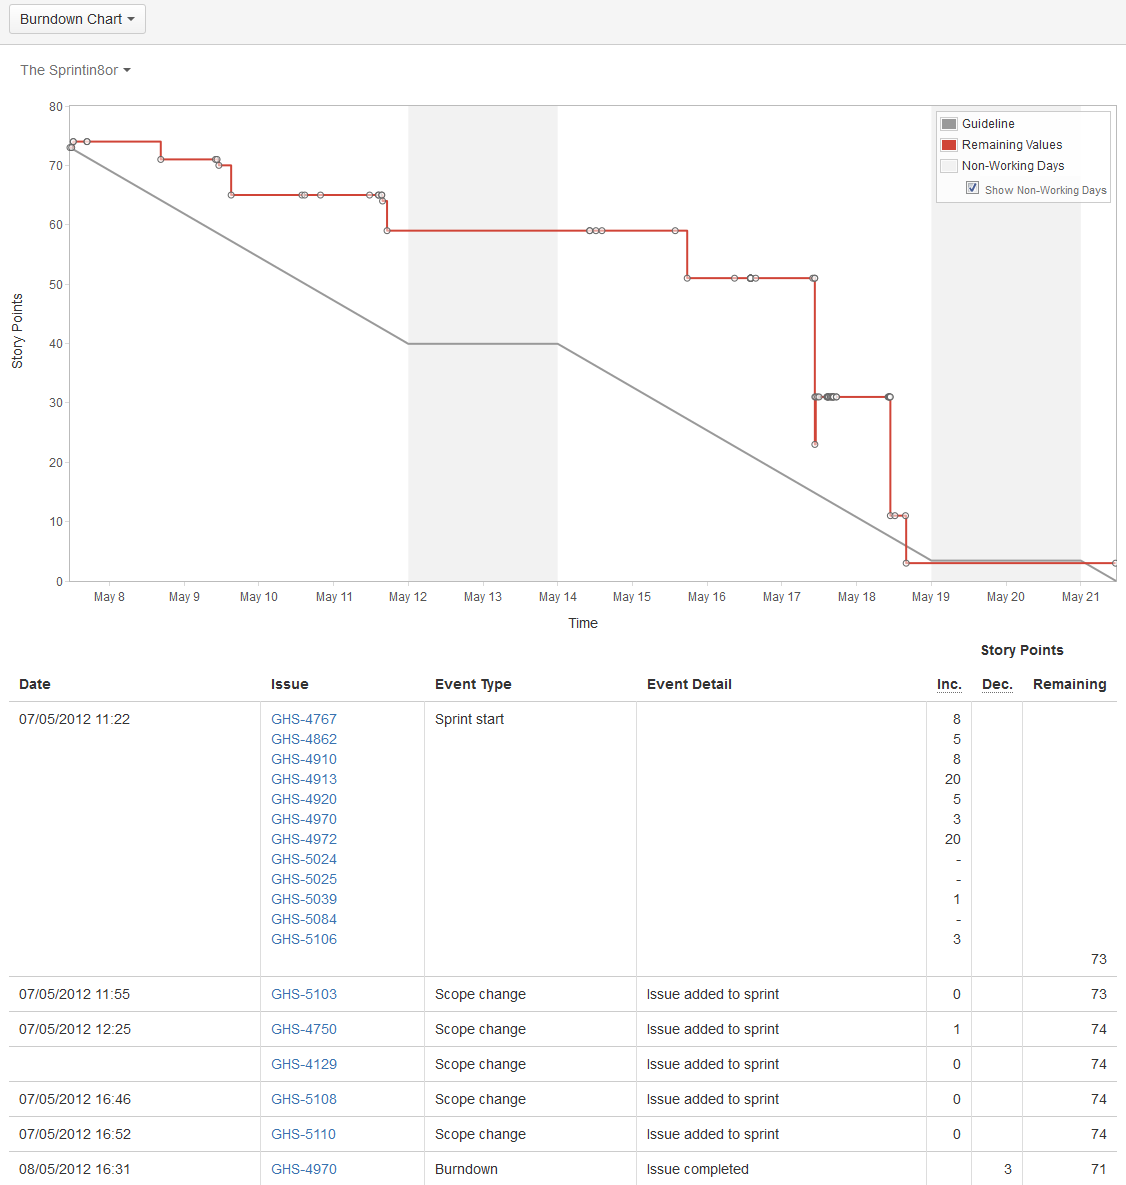
\includegraphics[scale=0.4]{img/burndown-chart.png}
	\caption{Screenshot: Burndown chart.} 
	\label{fig:burndown-chart}
\end{figure}

\textbf{Cumulative flow diagram}: A Cumulative Flow Diagram (CFD) is an area chart that shows the various statuses of work items for a product, version, or sprint. The horizontal x-axis in a CFD indicates time, and the vertical y-axis indicates cards (issues). Each colored area of the chart equates to a workflow status (i.e. a column on your board). This description is just due to completeness of content. Please refer to figure~\ref{fig:cumulative_flow_diagram} for further information.

\textbf{Epic report}: The Epic Report shows a list of complete, incomplete and unestimated issues in an epic. It is particularly useful for planning work for an epic that may extend over multiple sprints.
Use the Epic Report to understand the progress towards completing an epic over time, and to track the amount of remaining work that's incomplete or unestimated.

\begin{figure}[h]
	\centering
	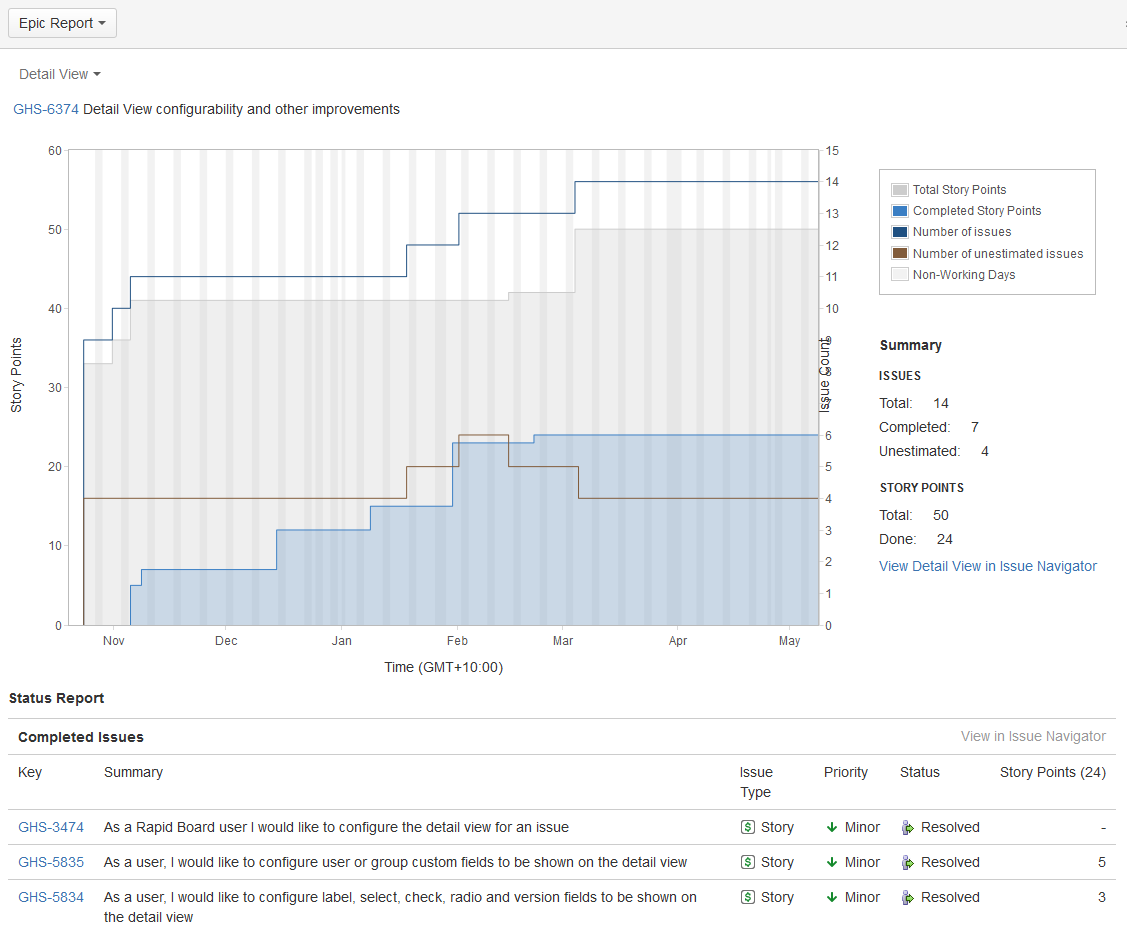
\includegraphics[scale=0.4]{img/epic-report.png}
	\caption{Screenshot: Epic report.} 
	\label{fig:epic-report}
\end{figure}

\textbf{Sprint report}: The sprint report shows the list of issues in each sprint. It is useful for your sprint retrospective meeting, and also for mid-sprint progress checks. If you have Confluence\footnote{\url{https://www.atlassian.com/software/confluence}} linked to your JIRA instance, you can also create and/or link Confluence pages to your sprint report. For example, you may want to create retrospective notes for the sprint. This only applies to Scrum boards.

\begin{figure}[h]
	\centering
	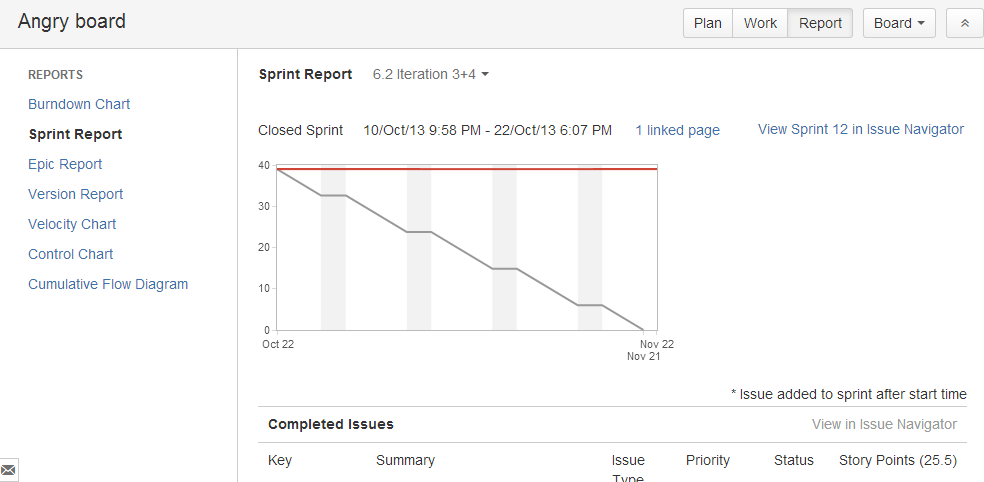
\includegraphics[scale=0.4]{img/sprintreport-linkedpages.png}
	\caption{Screenshot: Sprint report with linked Confluence pages.} 
	\label{fig:sprintreport-linkedpages}
\end{figure}

\textbf{Velocity chart}: The velocity chart shows the amount of value delivered in each sprint, enabling you to predict the amount of work the team can get done in future sprints. It is useful during your sprint planning meetings, to help you decide how much work you can feasibly commit to. This only applies to Scrum boards.

\begin{figure}[h]
	\centering
	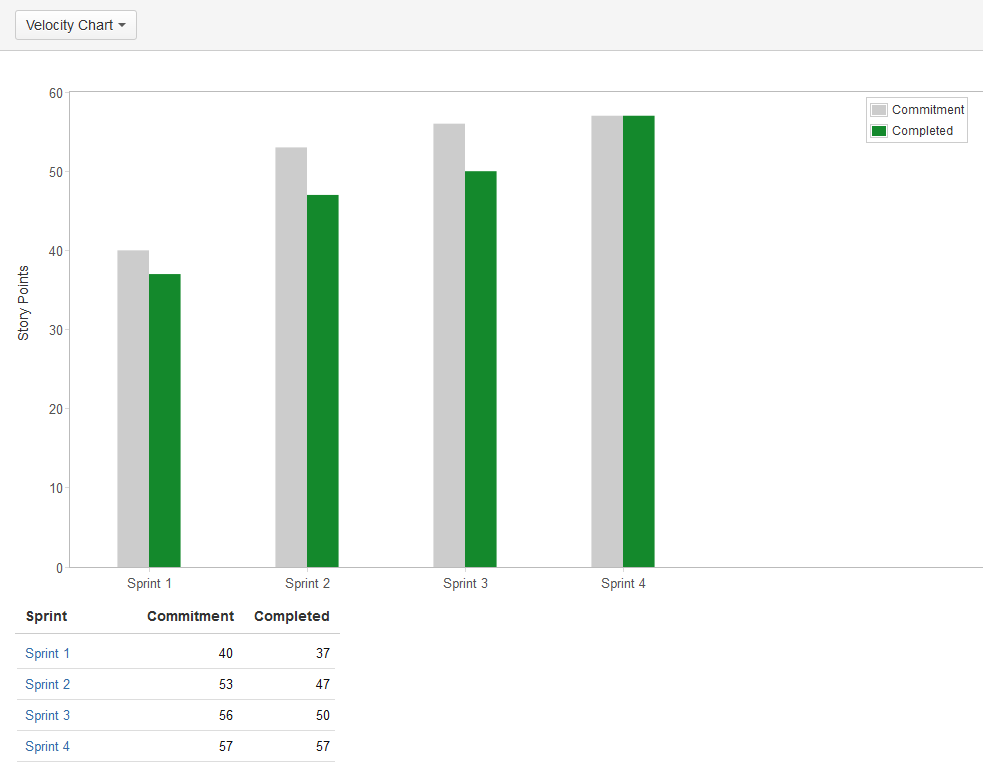
\includegraphics[scale=0.4]{img/velocity-chart.png}
	\caption{Screenshot: Velocity chart.} 
	\label{fig:velocity-chart}
\end{figure}

\textbf{Version report}: The version report shows your team's progress towards completion of a version. The version report also shows you the predicted Release Date, based on your team's average rate of progress (velocity) since the start of the version, and the estimated amount of work remaining. This only applies to Scrum boards.

\begin{figure}[h]
	\centering
	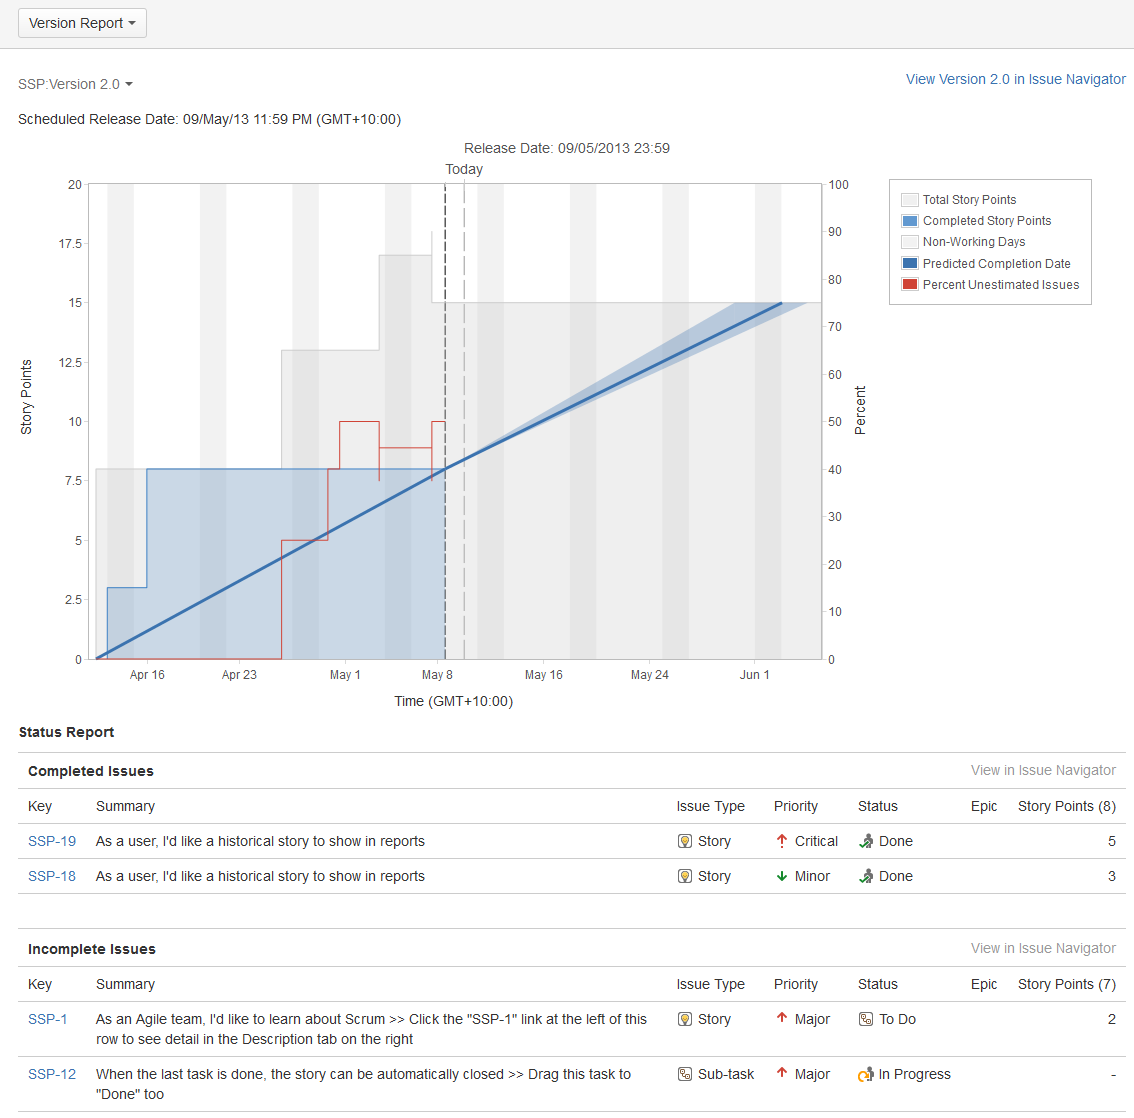
\includegraphics[scale=0.4]{img/version-report.png}
	\caption{Screenshot: Version report.} 
	\label{fig:version-report}
\end{figure}


	
	\listoffigures
	\bibliography{citations}

\end{document}